\chapter{Planejamento}
Conforme descrito no Capítulo \ref{cap:introducao}, este trabalho será constituído de cinco etapas.
Em um primeiro momento, a etapa de diagnóstico foi realizada e os sistemas relacionados e suas funcionalidades em comum foram apresentadas no Capítulo \ref{cap:sistemas_relacionados}. Em seguida, o objetivos do trabalho foram definidos. 

Para execução do trabalho foi estabelecido um cronograma que pode ser visto na Figura \ref{fig:cronograma}.
Foram contempladas as atividades iniciais realizadas e o planejamento para implementação da solução.
O desenvolvimento da API será por meio de um processo iterativo e incremental. 

\begin{figure}[h!]
\centering
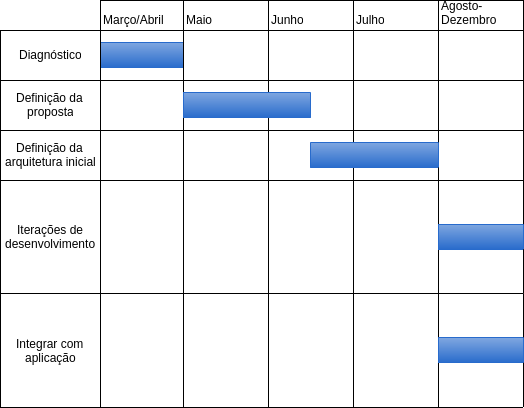
\includegraphics[scale=0.6]{figuras/cronograma.png}
\caption{Cronograma de execução}
\label{fig:cronograma}
\end{figure}

\section{Escopo}
Para alcançar os objetivos propostos foi feita uma avaliação do escopo da plataforma Empurrando Juntos, que é foco de contribuição deste trabalho.
Nessa avaliação foram mapeadas as entidades principais, seus atributos e os relacionamentos entre elas. Esse mapeamento pode ser visto na Figura \ref{fig:entidades}.

\begin{figure}[h!]
\centering
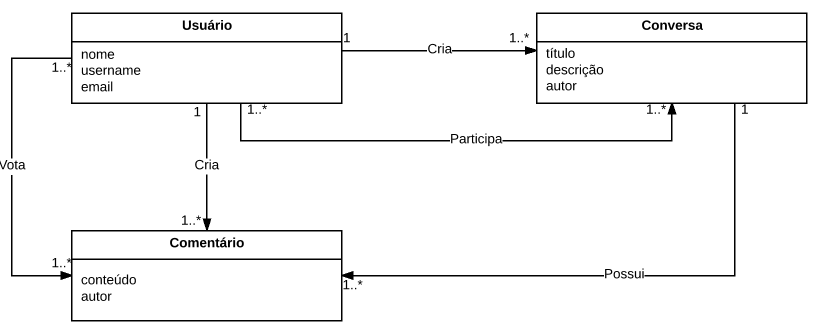
\includegraphics[scale=0.5]{figuras/entidades.png}
\caption{Entidades da API}
\label{fig:entidades}
\end{figure}

O funcionamento da plataforma basicamente contempla as três entidades apresentadas: Usuário, Conversa, Comentário. Um usuário cria uma conversa, a qual
pode possuir inúmeros comentários realizados por diversas pessoas. Em cada comentário é possível realizar um voto. O conceito de voto pode ser definido
para cada contexto de uso, um exemplo seria concordar ou discordar de um comentário. Cada pessoa que cria um comentário ou vota em um comentário
de uma conversa torna-se participante. 

A API terá como escopo o provimento de manutenção dessas entidades e seus relacionamentos (Participa e Vota, principalmente) por meio de serviços REST.


\section{Estrutura}

A API a ser criada faz parte de uma estrutura que será denominada como Pentano. O Pentano é constituído por dois módulos: o \textit{server}, que é o módulo da API
e o \textit{Math} que é o módulo responsável pela clusterização. Essa estrutura pode ser melhor visualizada na Figura \ref{fig:pentano}.

\begin{figure}[h!]
\centering
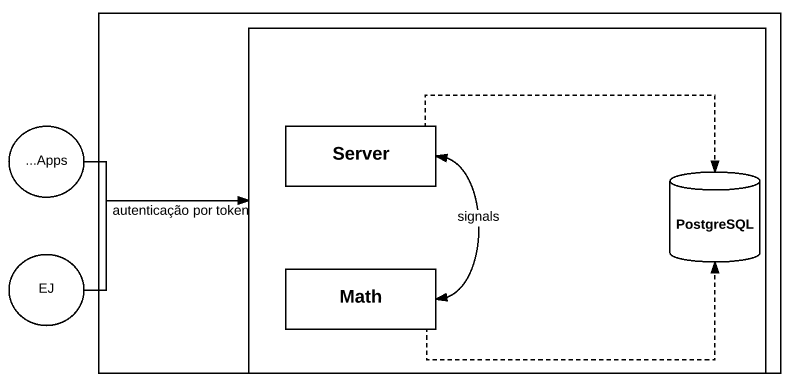
\includegraphics[scale=0.5]{figuras/esquema_pentano.png}
\caption{Estrutura do Pentano}
\label{fig:pentano}
\end{figure}


Para implementação do módulo \textit{Math} foi utilizada a linguagem Python. A API a ser implementada também utilizará a linguagem Python
juntamento com os \textit{frameworks} Django e Django Rest Framework.

\section{Resultados Esperados}

No final do trabalho é esperado uma API Rest que seja capaz de fornecer um serviço de participação com conversas, comentários
e votos que agrupe pessoas de acordo com os votos.

Com esse serviço, espera-se contribuir com a plataforma Empurrando Juntos através da implementação da parte servidor da 
arquitetura definida.

Dentro do contexto social, o objetivo é que a API possa contribuir no apoio à mulheres vítimas de violência, através
da promoção de discussões mais efetivas e a criação de uma rede de apoio entre mulheres que passam ou passaram por essa situação.








